\documentclass{article}
\usepackage{graphicx}
\usepackage{courier}
\usepackage{listings}
\usepackage{color}
\usepackage{cite}




\definecolor{dkgreen}{rgb}{0,0.6,0}
\definecolor{gray}{rgb}{0.5,0.5,0.5}
\definecolor{mauve}{rgb}{0.58,0,0.82}

\lstset{frame=tb,
  language=Java,
  aboveskip=3mm,
  belowskip=3mm,
  showstringspaces=false,
  columns=flexible,
  basicstyle={\small\ttfamily},
  numbers=none,
  numberstyle=\tiny\color{gray},
  keywordstyle=\color{blue},
  commentstyle=\color{dkgreen},
  stringstyle=\color{mauve},
  breaklines=true,
  breakatwhitespace=true,
  tabsize=3
}


\begin{document}

\title{A Title}


\maketitle

\begin{abstract}
  Current Research of GUI testing focus on event sequences.
  They can't cover code.
  We can.
\end{abstract}

\section{Introduction}\label{section:introduction}
this is a place holder sentense. \cite{jpf-awt}

\section{Example}

\begin{figure}
  \centering
  \caption{ticket example}
  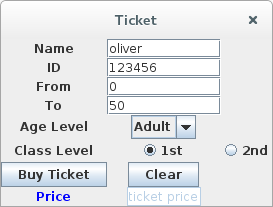
\includegraphics{./res/ticket.png}
\end{figure}

To demostrate  the importance of branch coverage testing of GUI applications, we will use a  \texttt{Ticket Seller} example application. Note that we borrowed the example from barad. Figure 1 shows the GUI of this \texttt{Ticket Seller} application.

This program is used to calculate ticket price according to different properties of the client, such as the class level, or age, or the travel distance. When the \texttt{Buy} button is clicked, the application check the \texttt{Name} and \texttt{ID} input, if the length of the \texttt{Name} string is less or equal than 3, or \texttt{ID} equals to some special string, then the application will display an error message and will not calculate any price. After checking the user information successfully, the application start to calculate the price as follows: read the user class input and set a coeffient for the price, read the user age to go to different pricing branch, read the start and dest input and calculate the distance of travelling, then calculate the price. We can see from the following code snippets that there should be many branches in the code to calculate ticket price for all kinds of clients.

\begin{lstlisting}
  int coeficient = (classLevel == TicketModel.FIRSTCLASS) ? 1 : 2;
  int dist = to - from;
  if (ageLevel == 1) {
    if (dist < 40) {
      price = 100 * coeficient;
    } else if (dist < 45) {
      price = 110 * coeficient;
    } else if (dist < 50) {
      price = 120 * coeficient;
    } else if (dist < 70) {
      price = 140 * coeficient;
    } else if (dist < 80) {
      price = 150 * coeficient;
    } else if (dist < 85) {
      price = 155 * coeficient;
    } else if (dist < 100) {
      price = 160 * coeficient;
    }
  }
\end{lstlisting}

One can not claim this kind of applications are well tested until all the branches has been covered during test stage.


\section{Inplementation}


Given an event sequence, our goal is to generate different user inputs for the event sequence to improve the code coverage of the test case.

besides generating user inputs, to make the tool easy to use we also set the following goals.
\begin{itemize}
  \item {auto instrument the aut, so the testing doesn't need manually set up symbolic variables in the source code. This is because sometimes the source code is not available, even if the source code is available, modify source code may add extra uncertainy to the product }
    \item{we automatically treat numerical inputs. GUI always treat user inputs as strings, it is the duty of the programmer to parse int from the string. }
      \end{itemize}



\par{\textit{A. Architecture}}
This project is implemented to test java GUI applications.
we build our work on top of two open source project: concolic testing project  \texttt{CATG} and gui testing project \texttt{GUITAR}.

\texttt{CATG}is a concolic unit testing engine for Java programs. The implementation uses ASM for instrumentation. ASM instrumentation instruments (see janala.instrument.) class files at runtime and dumps (see janala.logger.) to a file a log of all instructions executed by the program and all values loaded from local stacks and heaps. A concolic execution engine (see janala.interpreters.*) then takes the log and performs both symbolic and concrete interpretation of the logged instructions.

\texttt{GUITAR} supports a wide variety of model-based GUI testing techniques. The innovation lies in the architecture of GUITAR, which uses plug-ins to support flexibility and extensibility. Software developers and quality assurance engineers may use this architecture to create new toolchains, new workflows based on the toolchains, and plug in a variety of measurement tools to conduct GUI testing.

The first question is how to do with graphic user interface? It means unsupported functions in java built in library.
We first find that we can take advantage of concolic testing to test GUI applications. Since concolic testing using concrete execution when dealing with unsupported functions.

The second question is how to deal with user inputs. Since GUI applications are event driven, the program will idle to wait for user input. we come up with the idea that can we turn gui into a sequencial program? Fortunately we found guitar.

Since we have got the idea, we made baby step experiment. The results show that we our idea works. then the next problem is how to put the two projects together. we put jar files of two projects together, we use shell scripts to organize the whole process.

\textbf{auto instrument} when comes to test some industry programs, one find it hard to modify the source cdoe to add symbolic variables. Because we are not familiar with the source code at all. Since gui application inputs are fixed from the gui, why not we automate it?

The problem is catg can not handle getText(). when comes to getText(), catg goes to concrete execution. There are two possible apporach to overcome this problem. The first is to modify source code, manually replace getText by catg.readString(). The second is automatically replace bytecode of getText to a symbolicGetText() function which returns a symbolic variable.

We need a global symbolic variable table. So when symbolicGetText() is called, we return the arrcording value from the symbolic table.

We need to figure out which symbolic variable to return. We need some map from gui widget to a symbolic variable. The widget identifies is a string of accessibleName, which can be set by setAccessibleName or setLabelFor. This widget identifier is also used by guitar and jpf-awt to identify the gui widgets.

Since catg has different operation support for string and numbers. So what to do with user input which is logically a number like age or distance? java first use getText to get a string from userinput, then use parseInt to transform the string to int. But concolic catg will fall to concrete execution because it doesn't support parseInt. to overcome this problem, we modify catg to support parseInt.

Besides that we also need to figure out which user input should be numbers. To overcome this problem, we need user to wirte a configure file. The configure file should enumerate all the user inputs which should be treated symboliccally. Each entry should contail a tuple of widget accessibleName, parse function, date type, init value. For exmaple. To write such a configure file, the tester should know the accessible Name of the gui widgets, while this infomation usually can be provided by the programmers.

\textit{Name,getText,Sting,myName}

Once we have the configure file, we build a global symbolic table according to it. The symbolic table is a map, whose key is the accessibleName and value is the singleton symbolic object created by CATG.readString or CATG.readInt etc. Each entry in the configure file has exactly one entry in the symbolic table. We use singleton because for some unknown reason guitar will execute one event multiple times while replaying.

And once we have the configure file, we can instrument the aut bytecode, replace the gui widget by our symbolic table. When loading bytecode, when we find calling of getText, and the according object is one of the entries in the configure file, then this is where we should change to symbolic. Then we change the getText call to symbolicGetText call. Then the userinput does not come from widget any more, but comes from the symbolic one.

catg doens't support parseInt function. We add a key accessibleName  to StringVale when creating symbolic String. the key is used when identifying the parse Int caller object. if the object has the key, we can consult the configure file to confirm whether and how to treat it.

To add parseInt support, we modify catg. when the symbolic stack of catg execution the parseInt concrete command, it originally return a placeholder and the program becomes concrete execution. We modify catg, let it return a symbolic intValue which is created in the global symbolic table. Then the program can continue with symbolic execution.

Since we have introducted two symbolic values for a number user input, one is StringValue, one is IntValue. But the user only cares about the string one. So when finished execution, we need to transform the generated concrete user input of int to string, and overwrite the string. In other words, we need to hide our IntValue during the whole process. We do this by add the according int symbol to the string Value, when catg return with a StringValue, we checkout whether it contains such a symbol, if so we use the concrete value of IntValue according to the symbol to overwrite the string.


we use \texttt{ASM} framework to instrument.

\section{experiment}
We have tested ticket seller. We user guitar to generate testcase. Each guitar test case we have get up to 13 concrete inputs.


\section{Related Work}\label{section:relatedwork}
Current we support int value.
we are going to support float/double value.

Current we support textInput.
we are going to support radioButton. dropbox. textfield etc.

we are going to find more aut to test.


\bibliographystyle{unsrt}
\bibliography{paper}




\end{document}
